\documentclass[fleqn]{article}
\usepackage[utf8]{inputenc}
\usepackage[margin=2.5cm]{geometry}

% bibliography
\usepackage[round, sort&compress]{natbib}
\usepackage{har2nat}
\bibliographystyle{agsm}

% custom header/footer
\usepackage{fancyhdr}
\pagestyle{fancy}
\renewcommand{\headrulewidth}{0pt}
\fancyhf{}
\rfoot{\textsf{\thepage}}
\lfoot{\textsf{Suzie Brown}}

% miscellaneous formatting
\usepackage{xcolor}
\usepackage[font=small]{caption}
\usepackage{subcaption}
\usepackage{enumitem}

% tikz
\usepackage{tikz}
\usetikzlibrary{positioning}

% pseudocode
\usepackage{algorithm}
\usepackage{algorithmicx}
\usepackage{algpseudocode}

% maths / theorems
\usepackage{amsmath}
\usepackage{amssymb}
\usepackage{amsthm}
\newtheorem{thm}{Theorem}
\newtheorem{lemma}{Lemma}
\newtheorem{remark}{Remark}
\newtheorem{corollary}{Corollary}
\newtheorem{conj}{Conjecture}
\newtheorem{prop}{Proposition}
\theoremstyle{definition}
\newtheorem{defn}{Definition}

% useful math symbols
\newcommand{\N}{\mathbb{N}}
\newcommand{\Prob}{\mathbb{P}}
\newcommand{\E}{\mathbb{E}}
\newcommand{\V}{\operatorname{Var}}
\newcommand{\eqdist}{\overset{d}{=}}
\newcommand{\I}[1]{\mathbb{I}_{\{#1\}}}
\newcommand{\Ntoinfty}{\overset{N\to\infty}{\longrightarrow}}
\newcommand{\limNtoinfty}{\underset{N\to\infty}{\lim}}
\newcommand\indep{\protect\mathpalette{\protect\independenT}{\perp}}
\def\independenT#1#2{\mathrel{\rlap{$#1#2$}\mkern2mu{#1#2}}}

% distributions
\newcommand{\Cat}{\operatorname{Categorical}}
\newcommand{\Unif}{\operatorname{Uniform}}
\newcommand{\Mn}{\operatorname{Multinomial}}
\newcommand{\Bin}{\operatorname{Binomial}}

% project-specific symbols
\newcommand{\F}{\mathcal{F}_{t-1}}
\newcommand{\vt}[2][t]{\nu_{#1}^{(#2)}}
\newcommand{\wt}[2][t]{w_{#1}^{(#2)}}
\newcommand{\wbar}[2][t]{\bar{w}_{#1}^{(#2)}}
\newcommand{\vttilde}[2][t]{\tilde{\nu}_{#1}^{(#2)}}
\newcommand{\flnw}{\lfloor Nw_i \rfloor }

\title{Everything}
\author{Suzie Brown}
\date{\today}

\begin{document}
\maketitle
\thispagestyle{fancy}

\section{Notation}

\section{Summary of KJJS proof}

\section{Relaxing assumptions of KJJS theorem}

\section{Extension to conditional SMC}
\subsection{The conditional SMC update}\label{sec:condSMC_alg}
write something here...\\
referencing the CSMC algorithm...

\begin{algorithm}
\begin{algorithmic}[1]
\Require $N, T, \mu, \{K_t\}, \{g_t\}, y_{0:T}, x_{0:T}^*$
\For{$i \in \{1,\dots,N\}$} 
	\State Sample $X_0^{(i)} \sim \mu(\cdot)$ \Comment initialise
\EndFor
\State Sample $a_0^* \sim \Unif(\{1,\dots,N\})$
\State $X_0^{(a_0^*)} \gets x_0^*$
\For{$i \in \{1,\dots,N\}$}
	\State $w_0^{(i)} \gets g_0(X_0^{(i)})$
\EndFor
\State $W \gets \sum_{j=1}^N w_{0}^{(j)}$
	\For{$i \in \{1,\dots, N\}$}	
		\State $w_{0}^{(i)} \gets \frac{1}{W}w_{0}^{(i)}$ \Comment normalise weights
	\EndFor
\For{$t \in \{0,\dots, T-1\}$}
	\State Sample $a_t^{(1:N)} \sim \Cat(\{1,\dots,N\}, w_t^{(1:N)})$ \Comment resample particles
	\State Sample $a_{t+1}^* \sim \Unif(\{1,\dots,N\})$
	\State $a_t^{(a_{t+1}^*)} \gets a_t^*$
	\For{$i \in \{1,\dots,N\}$}
		\State Sample $X_{t+1}^{(i)} \sim K_{t+1}(X_t^{(a_t^{(i)})}, \cdot)$ \Comment propagate particles
	\EndFor
	\State $X_{t+1}^{(a_{t+1}^*)} \gets X_{t+1}^*$
	\For{$i \in \{1,\dots, N\}$}	
		\State $w_{t+1}^{(i)} \gets g_{t+1}(X_t^{(a_t^{(i)})} , X_{t+1}^{(i)})$ \Comment calculate weights
	\EndFor
	\State $W \gets \sum_{j=1}^N w_{t+1}^{(j)}$
	\For{$i \in \{1,\dots, N\}$}	
		\State $w_{t+1}^{(i)} \gets \frac{1}{W}w_{t+1}^{(i)}$ \Comment normalise weights
	\EndFor
\EndFor
\end{algorithmic}
\caption{Conditional SMC with multinomial resampling}
\label{alg:condSMC}
\end{algorithm}

\subsection{Conditional SMC genealogies}
\begin{thm}
Under the conditions of \citet[Lemma 3]{koskela2018}, the genealogy of any $n$ particles from a conditional SMC algorithm with multinomial resampling converges to Kingman's $n$-coalescent in the sense of finite-dimensional distributions, under the time-scaling defined in \eqref{eq:tau_tilde}.
\end{thm}

\begin{proof}
In the derivation of \eqref{eq:cNtilde} -- \eqref{eq:cNtilde2} we will make extensive use of the formula for factorial moments of the multinomial distribution given in \citet[p.67]{mosimann1962}:
\begin{equation} \label{eq:mn_moments}
\E[(X_i)_a(X_j)_b] = (n)_{a+b}\, p_i^a p_j^b
\end{equation}
where $(X_1,\dots X_k) \sim \Mn(n, \mathbf{p})$.
To apply this formula we need to write everything in terms of falling factorial powers. The required conversions are summarised in Table \ref{tab:fact_powers}.

In standard SMC with multinomial resampling, the marginal offspring distributions, conditioned on the filtration $\F$ generated by the previous offspring counts, are
\begin{equation*}
\vt{i} \eqdist \Bin (N, \wt{i}), \qquad i=1,\dots,N
\end{equation*}
where $\vt{i}$ is the number of offspring in generation $t+1$ of the $i$th particle in generation $t$, $N$ is the number of particles and $\wt{i}$ is the weight associated with the $i$th particle in generation $t$.

In conditional SMC we condition on the immortal trajectory surviving each resampling step. By exchangeability we can set without loss of generality that the immortal trajectory consists of particle 1 in each generation. At each resampling step, particle 1 must therefore choose particle 1 as its parent, while the remaining $N-1$ offspring are assigned multinomially to the $N$ possible parents. The marginal offspring distributions are then
\begin{align*}
& \vttilde{1} \eqdist 1 + \Bin(N-1, \wt{1}) \\
& \vttilde{i} \eqdist \Bin(N-1, \wt{i}), \qquad i=2,\dots,N.
\end{align*}
First let us consider the coalescence rate
\begin{equation*}
c_N(t) := \frac{1}{(N)_2} \sum_{i=1}^{N} (\vt{i})_2.
\end{equation*}
For standard SMC the expected value is, using the tower rule,
\begin{equation*}
\E[c_N(t) |\F] 
= \frac{1}{(N)_2} \sum_{i=1}^{N} \E\left[ \E[ (\vt{i})_2 ] |\F \right]
=\frac{1}{(N)_2} \sum_{i=1}^{N} \E\left[(N)_2 (\wt{i})^2 |\F \right] 
= \sum_{i=1}^{N} \E\left[(\wt{i})^2 |\F \right]
\end{equation*}
as stated in \citet[Remark 3]{koskela2018}.
In the case of conditional SMC we separate the first term (corresponding to the immortal particle) from the sum to get
\begin{align*}
\E[\tilde{c}_N(t) |\F] &= \frac{1}{(N)_2} \sum_{i=1}^{N} \E\left[ (\vttilde{i})_2 |\F \right] 
= \frac{1}{(N)_2} \E\left[ (\vttilde{1})_2 |\F \right] + \frac{1}{(N)_2}\sum_{i=2}^{N} \E\left[ (\vttilde{i})_2 |\F \right] \\
&= \frac{1}{(N)_2} \left\{ (N-1)_2\E[(\wt{1})^2 |\F] + 2(N-1)\E[\wt{1} |\F] + \sum_{i=2}^{N} (N-1)_2\E[(\wt{i})^2 |\F] \right\}\\
&= \frac{(N-1)_2}{(N)_2} \sum_{i=1}^{N} \E[(\wt{i})^2 |\F] + \frac{2(N-1)}{(N)_2} \E[\wt{1} |\F] \\
&= \frac{N-2}{N} \E[c_N(t) |\F] + \frac{2}{N} \E[\wt{1} |\F]
\end{align*}
which gives us \eqref{eq:cNtilde}.

\begin{table}
\centering
\begin{tabular}{r c l}
\hline
$x$ & $=$ & $(x)_1$ \\
$x^2$ & $=$ & $(x)_2 + (x)_1$ \\
$x^3$ & $=$ & $(x)_3 + 3(x)_2 + (x)_1$ \\
$x^4$ & $=$ & $(x)_4 + 6(x)_3 + 7(x)_2 + (x)_1$ \\
\hline
$xy$ & $=$ & $(x)_1(y)_1$ \\
$x^2y$ & $=$ & $(x)_2(y)_1 + (x)_1(y)_1$ \\
$xy^2$ & $=$ & $(x)_1(y)_2 + (x)_1(y)_1$ \\
$x^2y^2$ & $=$ & $(x)_2(y)_2 + (x)_2(y)_1 + (x)_1(y)_2 +  (x)_1(y)_1$ \\
\hline
$(x+1)_2$ & $=$ & $(x)_2 + 2(x)_1$ \\
$(x+1)^2$ & $=$ & $(x)_2 + 3(x)_1 + 1$ \\
$(x+1)_2(x+1)$ & $=$ & $(x)_3 + 5(x)_2 + 4(x)_1$ \\
$(x+1)_2^2$ & $=$ & $(x)_4 + 8(x)_3 + 14(x)_2 + 4(x)_1$ \\
\hline
\end{tabular}
\caption{Conversion of ordinary powers into falling factorial powers}
\label{tab:fact_powers}
\end{table}

An upper bound on the rate of super-binary mergers is given by
\begin{equation*}
D_N(t) := \frac{1}{N(N)_2} \sum_{i=1}^N (\vt{i})_2 \left( \vt{i} + \frac{1}{N} \sum_{j\neq i} (\vt{j})^2 \right).
\end{equation*}
In the standard case this quantity has expectation
\begin{align*}
\E[D_N(t) |\F] &= \frac{1}{N(N)_2} \sum_{i=1}^N \left\{ (N)_3\E[(\wt{i})^3 |\F] + 2(N)_2\E[(\wt{i})^2 |\F] \right\} \\
&\qquad + \frac{1}{N^2(N)_2} \sum_{i=1}^N \sum_{j\neq i} \left\{ (N)_4\E[(\wt{i})^2(\wt{j})^2 |\F] + (N)_3\E[(\wt{i})^2\wt{j} |\F] \right\}
\end{align*}
while in the conditional case, again separating the terms involving particle 1,
\begin{align*}
\tilde{D}_N(t) &= \frac{1}{N(N)_2} (\vttilde{1})_2 \left(\vttilde{1} + \frac{1}{N} \sum_{j\neq 1} (\vttilde{j})^2 \right)
+ \frac{1}{N(N)_2} \sum_{i\neq 1} (\vttilde{i})_2 \left( \vttilde{i} + \frac{1}{N}(\vttilde{1})^2 + \frac{1}{N} \sum_{1\neq j\neq i} (\vttilde{j})^2 \right)\\
&= \frac{1}{N(N)_2} \left\{ (\vttilde{1})_2\vt{1} + \frac{1}{N}\sum_{j\neq 1} (\vttilde{1})_2(\vttilde{j})^2 + \frac{1}{N}\sum_{i\neq 1} (\vttilde{i})_2(\vttilde{1})^2 \right\} \\
&\qquad + \frac{1}{N(N)_2} \sum_{i\neq 1} \left\{ (\vttilde{i})_2\vttilde{i} + \frac{1}{N}\sum_{1\neq j\neq i} (\vttilde{i})_2(\vttilde{j})^2 \right\} \\
&= \frac{1}{N(N)_2} \left\{ (\vttilde{1})_2\vttilde{1} + \frac{1}{N}\sum_{i\neq 1} \left( (\vttilde{1})_2(\vttilde{i})^2 + (\vttilde{i})_2(\vttilde{1})^2 \right) \right\} \\
&\qquad + \frac{1}{N(N)_2} \sum_{i\neq 1} \left\{ (\vttilde{i})_3 + 2(\vttilde{i})_2 + \frac{1}{N}\sum_{1\neq j\neq i} \left( (\vttilde{i})_2(\vttilde{j})_2 + (\vttilde{i})_2\vttilde{j} \right) \right\}
\end{align*}
and so by applying the moments from \eqref{eq:mn_moments} and Table \ref{tab:fact_powers} we find the expectation
\begin{align*}
&\E[\tilde{D}_N(t) |\F]= \\ 
&= \frac{1}{N(N)_2} \left\{ (N-1)_3\E[(\wt{1})^3 |\F] + 5(N-1)_2\E[(\wt{1})^2 |\F] +  4(N-1)\E[\wt{1} |\F] \right\} \\
&\qquad + \frac{1}{N^2(N)_2} \sum_{i=2}^N \left\{ 2(N-1)_4\E[(\wt{1})^2(\wt{i})^2 |\F] + (N-1)_3 \E[(\wt{1})^2\wt{i} |\F] \right.\\
&\qquad\qquad + 5(N-1)_3\E[\wt{1}(\wt{i})^2 |\F] 
 \left. +2(N-1)_2\E[\wt{1}\wt{i} |\F] + (N-1)_2\E[(\wt{i})^2 |\F] \right\} \\
&\qquad + \frac{1}{N(N)_2} \sum_{i=2}^N \left\{ 
(N-1)_3\E[(\wt{i})^3 |\F] + 2(N-1)_2\E[(\wt{i})^2 |\F] \right\} \\
&\qquad + \frac{1}{N^2(N)_2} \sum_{i=2}^N \sum_{1\neq j\neq i} \left\{ (N-1)_4\E[(\wt{i})^2(\wt{j})^2 |\F] + (N-1)_3\E[(\wt{i})^2\wt{j} |\F] \right\} \\
&= \frac{1}{N(N)_2} \sum_{i=1}^N \left\{ 
(N-1)_3\E[(\wt{i})^3 |\F] + 2(N-1)_2\E[(\wt{i})^2 |\F] \right\} \\
&\qquad + \frac{1}{N^2(N)_2} \sum_{i=1}^N \sum_{j\neq i} \left\{ (N-1)_4\E[(\wt{i})^2(\wt{j})^2 |\F] + (N-1)_3\E[(\wt{i})^2\wt{j} |\F] \right\} \\
&\qquad + \frac{1}{N(N)_2}\left\{ 3(N-1)_2\E[(\wt{1})^2 |\F] +  4(N-1)\E[\wt{1} |\F] \right\} \\
&\qquad+ \frac{1}{N^2(N)_2}\sum_{i=2}^N \left\{ 4(N-1)_3\E[\wt{1}(\wt{i})^2 |\F]
+2(N-1)_2\E[\wt{1}\wt{i} |\F] + (N-1)_2\E[(\wt{i})^2 |\F] \right\} \\
&\leq \E[D_N(t) |\F] + \frac{1}{N(N)_2} \left\{3(N-1)_2\E[(\wt{1})^2 |\F] +  4(N-1)\E[\wt{1} |\F] \right\} \\
&\qquad+ \frac{1}{N^2(N)_2}\sum_{i=2}^N \left\{ 4(N-1)_3\E[\wt{1}(\wt{i})^2 |\F] +2(N-1)_2\E[\wt{1}\wt{i} |\F] + (N-1)_2\E[(\wt{i})^2 |\F] \right\} \\
&\leq \E[D_N(t) |\F] + \frac{3}{N} \E[(\wt{1})^2 |\F] +  \frac{4}{N^2}\E[\wt{1} |\F] \\
&\qquad+ \frac{4}{N}\sum_{i=2}^N \E[\wt{1}(\wt{i})^2 |\F] +\frac{2}{N^2}\sum_{i=2}^N \E[\wt{1}\wt{i} |\F] + \frac{1}{N^2} \sum_{i=2}^N \E[(\wt{i})^2 |\F] 
\end{align*}
The second line of the first equality relies on multiplying the relevant terms in Table \ref{tab:fact_powers}. For the second equality we recombine the terms in particle 1 into the sum. The inequalities follow by bounding e.g.\ $N-1$ by $N$, and identifying the first two lines with $\E[D_N(t) |\F]$. This gives us the inequality \eqref{eq:DNtilde}.

We also need control of the squared coalescence rate:
\begin{align*}
c_N(t)^2 &= \frac{1}{(N)_2^2} \left( \sum_{i=1}^N (\vt{i})_2\right)^2 = \frac{1}{(N)_2^2} \left\{ \sum_{i=1}^N \E[(\vt{i})_2^2] + \sum_{i=1}^N\sum_{j\neq i} \E[(\vt{i})_2(\vt{j})_2] \right\}
\end{align*}
A bound on its expected value is proved in \citet{koskela2018}, but here we will use a different, more explicit bound to allow direct comparison between the standard and conditional cases.
For standard SMC we have:
\begin{align*}
\E[c_N(t)^2 |\F] &= \frac{1}{(N)_2^2} \left\{ (N)_4 \sum_{i=1}^N \E[(\wt{i})^4 |\F] + 4(N)_3 \sum_{i=1}^N \E[(\wt{i})^3 |\F] + 2(N)_2 \sum_{i=1}^N \E[(\wt{i})^2 |\F] \right\} \\
&\qquad + \frac{1}{(N)_2^2}(N)_4 \sum_{i=1}^N\sum_{j\neq i} \E[(\wt{i})^2(\wt{j})^2 |\F] \\
&= \frac{1}{(N)_2} \left\{ (N-2)_2 \sum_{i=1}^N \E[(\wt{i})^4 |\F] + 4(N-2) \sum_{i=1}^N \E[(\wt{i})^3 |\F] + 2 \sum_{i=1}^N \E[(\wt{i})^2 |\F] \right. \\
&\hspace{230pt}+ \left. (N-2)_2 \sum_{i=1}^N\sum_{j\neq i} \E[(\wt{i})^2(\wt{j})^2 |\F] \right\}
\end{align*}
For conditional SMC, we again separate the terms involving particle 1:
\begin{align*}
\tilde{c}_N(t)^2 &= \frac{1}{(N)_2^2} \left\{ \sum_{i=1}^N \E[(\vttilde{i})_2^2] 
+ \sum_{i=1}^N\sum_{j\neq i} \E[(\vttilde{i})_2(\vttilde{j})_2] \right\} \\
&= \frac{1}{(N)_2^2} \left\{ \sum_{i=2}^N \E[(\vttilde{i})_2^2] +\E[(\vttilde{1})_2^2] 
+ \sum_{i=2}^N\sum_{1\neq j\neq i} \E[(\vttilde{i})_2(\vttilde{j})_2] + 2\sum_{i=2}^N \E[(\vttilde{1})_2(\vttilde{i})_2] \right\} \\
\end{align*}
and then use the same techniques as for $\tilde{D}_N(t)$ to calculate the expectation:
\begin{align*}
&\E[\tilde{c}_N(t)^2 |\F]= \\ 
&= \frac{1}{(N)_2^2} \left\{ (N-1)_4 \sum_{i=2}^N \E[(\wt{i})^4 |\F] + 4(N-1)_3 \sum_{i=2}^N \E[(\wt{i})^3 |\F] + 2(N-1)_2 \sum_{i=2}^N \E[(\wt{i})^2 |\F] \right\}  \\
&\qquad + \frac{1}{(N)_2^2} \left\{ (N-1)_4\E[(\wt{1})^4 |\F] + 8(N-1)_3\E[(\wt{1})^3 |\F] + 14(N-1)_2\E[(\wt{1})^2 |\F] \right\} \\
&\qquad +  \frac{1}{(N)_2^2}4(N-1)\E[\wt{1} |\F]
+ \frac{1}{(N)_2^2}  (N-1)_4 \sum_{i=2}^N \sum_{1\neq j \neq i} \E[(\wt{i})^2(\wt{j})^2 |\F] \\
&\qquad +\frac{2}{(N)_2^2} \sum_{i=2}^N \left( (N-1)_4 \E[(\wt{1})^2(\wt{i})^2 |\F] + 2(N-1)_3 \E[\wt{1}(\wt{i})^2 |\F] \right) \\
&= \frac{1}{(N)_2^2} \left\{ (N-1)_4 \sum_{i=1}^N \E[(\wt{i})^4 |\F] + 4(N-1)_3 \sum_{i=1}^N \E[(\wt{i})^3 |\F] + 2(N-1)_2 \sum_{i=1}^N \E[(\wt{i})^2 |\F] \right\} \\
&\qquad + \frac{(N-1)_4}{(N)_2^2} \sum_{i=1}^N\sum_{j\neq i} \E[(\wt{i})^2(\wt{j})^2 |\F] \\
&\qquad +\frac{1}{(N)_2^2} \left\{ 4(N-1)_3 \E[(\wt{1})^3 |\F] + 12(N-1)_2\E[(\wt{1})^2 |\F] + 4(N-1)\E[\wt{1} |\F] \right\} \\
&\qquad +\frac{1}{(N)_2^2} \left\{ 4(N-1)_3 \sum_{i=2}^N \E[\wt{1}(\wt{i})^2 |\F] \right\} \\
&\leq  \E[c_N(t)^2 |\F] + \frac{1}{(N)_2^2} \left\{4(N-1)_3 \E[(\wt{1})^3 |\F] + 12(N-1)_2 \E[(\wt{1})^2 |\F] \right\}\\
&\qquad +\frac{1}{(N)_2^2} \left\{ 4(N-1)\E[\wt{1} |\F]
+ 4(N-1)_3 \sum_{i=2}^N \E[\wt{1}(\wt{i})^2 |\F] \right\} \\
&\leq \E[c_N(t)^2 |\F] + \frac{4}{N}\E[(\wt{1})^3 |\F] + \frac{12}{N^2} \E[(\wt{1})^2 |\F] + \frac{4}{N(N)_2} \E[\wt{1} |\F]\\
&\qquad + \frac{4}{N} \sum_{i=2}^N \E[\wt{1}(\wt{i})^2 |\F]
\end{align*}
The conditions (18) and (19) of \citet[Lemma 3]{koskela2018} give us control over the weights so that we have $\wt{i} = O(1)$ for all $i$. Under these conditions, in the limit as $N\to\infty$, the three modified expectations derived above simplify to:
\begin{align*}
& \E[\tilde{c}_N(t) |\F] \leq \E[c_N(t) |\F] + O(N^{-2}) \\
& \E[\tilde{D}_N(t) |\F] \leq \E[D_N(t) |\F] +O(N^{-3}) \\
& \E[\tilde{c}_N(t)^2 |\F] \leq \E[c_N(t)^2 |\F] + O(N^{-3})
\end{align*}
This shows that each of these quantities for conditional SMC is bounded above by the corresponding standard SMC quantity, plus some vanishing error term. This will allow us to apply \citet[Theorem 1]{koskela2018}, as we will show in the following.

Next we apply the result of \citet[Lemma 3]{koskela2018}, so that for our modified quantity $\tilde{c}_N(t)$ we have the upper bound:
\begin{align}\label{eq:cN_upper}
\E[\tilde{c}_N(t) |\F] &= \frac{N-2}{N} \E[c_N(t) |\F] + \frac{2}{N} \E[\wt{1} |\F] \notag\\
& \leq \E[c_N(t) |\F] + \frac{2}{N} \E[\wt{1} |\F] \notag\\
&\leq \frac{a^4}{N\varepsilon^4} +  \frac{2}{N} \E[\wt{1} |\F] \notag\\
&= \frac{a^4}{N\varepsilon^4} + O(N^{-2})
\end{align}
and lower bound:
\begin{align}\label{eq:cN_lower}
\E[\tilde{c}_N(t) |\F] &= \frac{N-2}{N} \E[c_N(t) |\F] + \frac{2}{N} \E[\wt{1} |\F] \notag\\
& \geq  \frac{N-2}{N}\frac{\varepsilon^4}{Na^4} + O(N^{-2}) \notag\\
& = \frac{\varepsilon^4}{Na^4} - \frac{2\varepsilon^4}{N^2a^4} + O(N^{-2}) \notag\\
& = \frac{\varepsilon^4}{Na^4} + O(N^{-2})
\end{align}
corresponding to (22) in \citet{koskela2018}, except for the addition of a vanishing error term.
Furthermore, we obtain for the other quantities (where the constant $C$ may change from one line to the next):
\begin{align}\label{eq:DN_upper}
\E[\tilde{D}_N(t) |\F] &\leq \E[D_N(t) |\F] + O(N^{-3}) \notag\\
&\leq \frac{C}{N} \E[c_N(t) |\F] + O(N^{-3}) \notag\\
&= \frac{C}{N} \E[\tilde{c}_N(t) |\F] + O(N^{-3})
\end{align}
and
\begin{align}\label{eq:cN2_upper}
\E[\tilde{c}_N(t)^2 |\F] &\leq \E[c_N(t)^2 |\F] + O(N^{-3}) \notag\\
&\leq \frac{C}{N} \E[c_N(t) |\F] + O(N^{-3}) \notag\\
&= \frac{C}{N} \E[\tilde{c}_N(t) |\F] + O(N^{-3})
\end{align}
according to equations (20) and (21) in \citet{koskela2018}, again with additional error terms.

Now let us define the time-scaling:
\begin{equation*}
\tilde{\tau}_N(t) := \min\left\{ s\geq 1 : \sum_{r=1}^s \tilde{c}_N(r) \geq t \right\}
\end{equation*}
which is a generalised inverse of $\tilde{c}_N(t)$ and thus satisfies the property:
\begin{equation}\label{eq:sum_tau_cN_upperlower}
t-s-1 \leq \sum_{r=\tilde{\tau}_N(s)+1}^{\tilde{\tau}_N(t)} \tilde{c}_N(r) \leq t-s +1 .
\end{equation}

We are finally ready to verify the conditions of \citet[Theorem 1]{koskela2018}. The conditions are the following.
\begin{description}
\item[(Standing Assumption)] The conditional distribution of parental indices $a_t^{(1:N)}$ given offspring counts $v_t^{(1:N)}$ is uniform over all valid assignments.
\item[(A)] $\limNtoinfty \E\left[ \sum_{r=\tilde{\tau}_N(s)+1}^{\tilde{\tau}_N(t)} \tilde{D}_N(r) \right] =0$
\item[(B)] $\limNtoinfty \E[\tilde{c}_N(t)] =0$
\item[(C)] $\limNtoinfty \E\left[ \sum_{r=\tilde{\tau}_N(s)+1}^{\tilde{\tau}_N(t)} \tilde{c}_N(r)^2 \right] =0$
\item[(D)] $\E[\tilde{\tau}_N(t) - \tilde{\tau}_N(s)] \leq C_{t,s}N$
\end{description}
These five conditions are verified below.
\begin{description}
\item{\textbf{(Standing Assumption)}} This holds by the exchangeability of offspring assignments arising from Algorithm \ref{alg:condSMC}.
\item{\textbf{(B)}} Using \eqref{eq:cN_upper} and applying the tower rule, we find
\begin{equation*}
\E[\tilde{c}_N(t)] = \E[\E[\tilde{c}_N(t) |\F]] \leq \frac{a^4}{N\varepsilon^4} + O(N^{-2}) \Ntoinfty 0
\end{equation*}
\item{\textbf{(C)}} Using \citet[Lemma 2]{koskela2018} along with \eqref{eq:cN2_upper} and the upper bound in \eqref{eq:sum_tau_cN_upperlower},
\begin{align*}
\E\left[ \sum_{r=\tilde{\tau}_N(s)+1}^{\tilde{\tau}_N(t)} \tilde{c}_N(r)^2 \right] 
&= \E\left[ \sum_{r=\tilde{\tau}_N(s)+1}^{\tilde{\tau}_N(t)} \E[\tilde{c}_N(r)^2 |\F] \right]
\leq  \E\left[ \sum_{r=\tilde{\tau}_N(s)+1}^{\tilde{\tau}_N(t)} \left( \frac{C}{N}\E[\tilde{c}_N(t) |\F] + O(N^{-3})\right) \right] \\
&= \frac{C}{N}  \E\left[ \sum_{r=\tilde{\tau}_N(s)+1}^{\tilde{\tau}_N(t)} \E[\tilde{c}_N(t) |\F] \right] + O(N^{-2})
= \frac{C}{N}  \E\left[ \sum_{r=\tilde{\tau}_N(s)+1}^{\tilde{\tau}_N(t)} \tilde{c}_N(r) \right] + O(N^{-2}) \\
&\leq \frac{C}{N}(t-s+1) + O(N^{-2}) \Ntoinfty 0
\end{align*}
\item{\textbf{(A)}} The above calculation replacing \eqref{eq:cN2_upper} with \eqref{eq:DN_upper} yields
\begin{align*}
\E\left[ \sum_{r=\tilde{\tau}_N(s)+1}^{\tilde{\tau}_N(t)} \tilde{D}_N(r) \right]
&= \E\left[ \sum_{r=\tilde{\tau}_N(s)+1}^{\tilde{\tau}_N(t)} \E[\tilde{D}_N(r) |\F] \right] \\
&\leq  \E\left[ \sum_{r=\tilde{\tau}_N(s)+1}^{\tilde{\tau}_N(t)} \left( \frac{C}{N}\E[\tilde{c}_N(t) |\F] + O(N^{-3})\right) \right] 
\Ntoinfty 0
\end{align*}
\item{\textbf{(D)}} Using \eqref{eq:cN_lower}, the upper bound in \eqref{eq:sum_tau_cN_upperlower} and \citet[Lemma 2]{koskela2018},
\begin{align*}
\E[\tilde{\tau}_N(t) - \tilde{\tau}_N(s)] 
&= \E\left[ \sum_{r=\tilde{\tau}_N(s)+1}^{\tilde{\tau}_N(t)} 1 \right] 
= \E\left[ \sum_{r=\tilde{\tau}_N(s)+1}^{\tilde{\tau}_N(t)} \frac{\E[\tilde{c}_N(r) |\F]}{\E[\tilde{c}_N(r) |\F]} \right] 
\leq \E\left[ \sum_{r=\tilde{\tau}_N(s)+1}^{\tilde{\tau}_N(t)} \frac{\E[\tilde{c}_N(r) |\F]}{\frac{\varepsilon^4}{Na^4}+O(N^{-2})} \right] \\
&= \frac{1}{\frac{\varepsilon^4}{Na^4}+O(N^{-2})} \E\left[ \sum_{r=\tilde{\tau}_N(s)+1}^{\tilde{\tau}_N(t)} \E[\tilde{c}_N(r) |\F] \right] 
= \frac{1}{\frac{\varepsilon^4}{Na^4}+O(N^{-2})} \E\left[ \sum_{r=\tilde{\tau}_N(s)+1}^{\tilde{\tau}_N(t)} \tilde{c}_N(r) \right] \\
&\leq \frac{t-s+1}{\frac{\varepsilon^4}{Na^4	}+O(N^{-2})} = \frac{(t-s+1)a^4 N}{\varepsilon^4 + O(N^{-1})} 
= (t-s+1)\frac{a^4}{\varepsilon^4}N + O(1)
\end{align*}
where the last equality follows by a Taylor expansion of $(\frac{\varepsilon^4}{Na^4	}+O(N^{-2}))^{-1}$.\\
Similarly we derive a lower bound using \eqref{eq:cN_upper}, the lower bound in \eqref{eq:sum_tau_cN_upperlower} and \citet[Lemma 2]{koskela2018}:
\begin{align*}
\E[\tilde{\tau}_N(t) - \tilde{\tau}_N(s)] 
&= \E\left[ \sum_{r=\tilde{\tau}_N(s)+1}^{\tilde{\tau}_N(t)} 1 \right] 
= \E\left[ \sum_{r=\tilde{\tau}_N(s)+1}^{\tilde{\tau}_N(t)} \frac{\E[\tilde{c}_N(r) |\F]}{\E[\tilde{c}_N(r) |\F]} \right] 
\geq \E\left[ \sum_{r=\tilde{\tau}_N(s)+1}^{\tilde{\tau}_N(t)} \frac{\E[\tilde{c}_N(r) |\F]}{\frac{a^4}{N\varepsilon^4}+O(N^{-2})} \right] \\
&= \frac{1}{\frac{a^4}{N\varepsilon^4}+O(N^{-2})} \E\left[ \sum_{r=\tilde{\tau}_N(s)+1}^{\tilde{\tau}_N(t)} \E[\tilde{c}_N(r) |\F] \right] 
= \frac{1}{\frac{a^4}{N\varepsilon^4}+O(N^{-2})} \E\left[ \sum_{r=\tilde{\tau}_N(s)+1}^{\tilde{\tau}_N(t)} \tilde{c}_N(r) \right] \\
&\geq \frac{t-s-1}{\frac{a^4}{N\varepsilon^4}+O(N^{-2})} = \frac{(t-s-1)\varepsilon^4 N}{a^4 + O(N^{-1})} 
= (t-s-1)\frac{\varepsilon^4}{a^4}N + O(1)
\end{align*}
Therefore we have as required
\begin{equation*}
\E[\tilde{\tau}_N(t) - \tilde{\tau}_N(s)] \sim C_{t,s} N
\end{equation*}
as $N\to\infty$.
\end{description}
\end{proof}

\subsection{With the updated theorem assumptions...}
\begin{thm}\label{thm:mn_newassns}
Under the time scaling of \citet[Theorem 1]{koskela2018} and the conditions of \citet[Lemma 3]{koskela2018}, genealogies of SMC algorithms with multinomial resampling converge to Kingman's $n$-coalescent in the sense of finite-dimensional distributions as $N\to\infty$.
\end{thm}

\begin{proof}
The standing assumption holds by exchangeability of the Multinomial distribution.
We also need to show that there exists a deterministic sequence $(b_N)_{N\in\N}$ such that $\limNtoinfty b_N =0$ and
\begin{equation}\label{eq:csmc_ratiobound}
\frac{\frac{1}{(N)_3}{\sum_{i=1}^N \E[(\vt{i})_3 |\F}}{\frac{1}{(N)_2} \sum_{i=1}^N \E[(\vt{i})_2 |\F]} \leq b_N
\end{equation}
for all $N \in \N$. 
For the denominator, we apply \citet[Lemma 3]{koskela2018} directly to obtain, for some constants $a\geq \varepsilon\geq0$,
\begin{equation*}
\sum_{i=1}^N \E[(\vt{i})_2 |\F] \geq \frac{(N)_2 \varepsilon^4}{Na^4}
\end{equation*}
For the numerator, we use that $\vt{i} \longrightarrow (\vt{i})_3$ is $\{i\}$-increasing, along with the argument from the proof of \citet[Lemma 3]{koskela2018}, to obtain
\begin{equation*}
\sum_{i=1}^N \E[(\vt{i})_3 |\F] \leq \sum_{i=1}^N  \E[(\tilde{a}_t^{(i)})_3]
\end{equation*}
where
\begin{equation}
\tilde{a}_t^{(j)} \sim^{iid} \Cat \left( \left(\frac{a}{\varepsilon}\right)^{\I{i=1}-\I{i\neq 1}}, \left(\frac{a}{\varepsilon}\right)^{\I{i=2}-\I{i\neq 2}}, \dots, \left(\frac{a}{\varepsilon}\right)^{\I{i=N}-\I{i\neq N}} \right)
\end{equation}
We can calculate the expectation for $\tilde{a}_t^{(1:N)}$, so we obtain
\begin{align*}
\sum_{i=1}^N \E[(\vt{i})_3 |\F] &\leq 
(N)_3 \left( \frac{1}{(N-1)\varepsilon/a + a/\varepsilon} \right)^3 \left[ (N-1)\left(\frac{\varepsilon}{a}\right)^3 + \left(\frac{a}{\varepsilon}\right)^3 \right] \\
&= \frac{(N)_3}{\left((N-1)\varepsilon/a + a/\varepsilon\right)^3}\left(a^6 + (N-1)\varepsilon^6\right) \\
&\leq \frac{(N)_3}{N^3\varepsilon^6} (Na^6) = \frac{(N)_3}{N^2} \frac{a^6}{\varepsilon^6}
\end{align*}
where the last inequality follows because $a\geq \varepsilon$.
Putting these together, we can bound the ratio above by
\begin{equation}
b_N := \frac{(N)_3 \frac{(N)_3}{N^2} \frac{a^6}{\varepsilon^6}}{(N)_2 \frac{(N)_2 \varepsilon^4}{Na^4}} = \frac{1}{N}\frac{a^{10}}{\varepsilon^{10}} \quad \Ntoinfty 0
\end{equation}
We conclude the result by applying Theorem ? [the KJJS Thm1 with updated assns].
\end{proof}

\begin{thm}\label{thm:CSMC_newassns}
Under the time scaling of \citet[Theorem 1]{koskela2018} and the conditions of \citet[Lemma 3]{koskela2018}, genealogies of conditional SMC algorithms with multinomial resampling converge to Kingman's $n$-coalescent in the sense of finite-dimensional distributions as $N\to\infty$.
\end{thm}

\begin{proof}
Denote the vector of particle weights $\wt{1:N} = (\wt{1}, \wt{2}, \dots, \wt{N})$.
Let $\vttilde{1:N} = (\vttilde{1}, \vttilde{2}, \dots, \vttilde{N})$ denote the associated offspring counts under conditional SMC. Assuming WLOG that the immortal particle is particle 1, the offspring counts are distributed according to
\begin{equation*}
\vttilde{1:N} \mid \wt{1:N} \eqdist (1,0,0,\dots, 0) + \Mn(N-1, \wt{1:N})
\end{equation*}
The standing assumption holds by exchangeability of the offspring assignments in Algorithm \ref{alg:condSMC}. 
As before, we need to show that
\begin{equation}\label{eq:csmc_ratiobound}
\frac{\frac{1}{(N)_3}{\sum_{i=1}^N \E[(\vttilde{i})_3 |\F}}{\frac{1}{(N)_2} \sum_{i=1}^N \E[(\vttilde{i})_2 |\F]} \leq b_N
\end{equation}
for some deterministic sequence $b_N \limNtoinfty 0$. For the denominator, we find
\begin{align*}
{\sum_{i=1}^N \E[(\vttilde{i})_2 |\F}
&=  \E\left[ (\vttilde{1})_2 |\F \right] + \sum_{i=2}^{N} \E\left[ (\vttilde{i})_2 |\F \right] \\
&= (N-1)_2\E[(\wt{1})^2 |\F] + 2(N-1)\E[\wt{1} |\F] + \sum_{i=2}^{N} (N-1)_2\E[(\wt{i})^2 |\F] \\
&= (N-1)_2 \sum_{i=1}^{N} \E[(\wt{i})^2 |\F] + 2(N-1) \E[\wt{1} |\F] 
\end{align*}
using that $(X+1)_2 = (X)_2 + 2(X)_1$ and the factorial moments of the Multinomial distribution \citep{mosimann1962}.
For the numerator, we have
\begin{align*}
{\sum_{i=1}^N \E[(\vttilde{i})_3 |\F}
&=  \E\left[ (\vttilde{1})_3 |\F \right] + \sum_{i=2}^{N} \E\left[ (\vttilde{i})_3 |\F \right] \\
&= (N-1)_3\E[(\wt{1})^3 |\F] + 3(N-1)_2\E[(\wt{1})^2 |\F] + \sum_{i=2}^{N} (N-1)_3\E[(\wt{i})^3 |\F] \\
&= (N-1)_3 \sum_{i=1}^{N} \E[(\wt{i})^3 |\F] + 3(N-1)_2 \E[(\wt{1})^2 |\F] 
\end{align*}
using similarly that $(X+1)_3 = (X)_3 + 3(X)_2$.
Combining these expressions, the ratio in \eqref{eq:csmc_ratiobound} becomes
\begin{align*}
\frac{\frac{1}{(N)_3}{\sum_{i=1}^N \E[(\vttilde{i})_3 |\F}}{\frac{1}{(N)_2} \sum_{i=1}^N \E[(\vttilde{i})_2 |\F]}
&= \frac{1}{N-2} \frac{(N-1)_3 \sum_{i=1}^{N} \E[(\wt{i})^3 |\F] + 3(N-1)_2 \E[(\wt{1})^2 |\F] }{(N-1)_2 \sum_{i=1}^{N} \E[(\wt{i})^2 |\F] + 2(N-1) \E[\wt{1} |\F]} \\
&\leq \frac{1}{N-2} \frac{(N-1)_3 \sum_{i=1}^{N} \E[(\wt{i})^3 |\F]}{(N-1)_2 \sum_{i=1}^{N} \E[(\wt{i})^2 |\F]} + \frac{1}{N-2} \frac{3(N-1)_2 \E[(\wt{1})^2 |\F]}{(N-1)_2 \sum_{i=1}^{N} \E[(\wt{i})^2 |\F]} \\
&\leq \frac{1}{N-2} \frac{(N-1)_3 \sum_{i=1}^{N} \E[(\wt{i})^3 |\F]}{(N-1)_2 \sum_{i=1}^{N} \E[(\wt{i})^2 |\F]} + \frac{1}{N-2} \frac{3(N-1)_2 \E[(\wt{1})^2 |\F]}{(N-1)_2 \E[(\wt{1})^2 |\F]} \\
&<  \frac{1}{N-2} \frac{\sum_{i=1}^{N} \E[(\vt{i})_3 |\F]}{\sum_{i=1}^{N} \E[(\vt{i})_2 |\F]} + \frac{3}{N-2}
\end{align*}
where the last inequality comes from $\frac{(N-1)_3}{(N-1)_2} = N-3 < N-2 = \frac{(N)_3}{(N)_2}$.
Then, using Theorem \ref{thm:mn_newassns}, we can bound this by
\begin{equation*}
b_N := \frac{1}{N}\frac{a^6}{\varepsilon^6} + \frac{3}{N-2} \quad \Ntoinfty 0
\end{equation*}
as required, where $a$ and $\varepsilon$ are constants defined in the conditions of \citet[Lemma 3]{koskela2018}.
We conclude the result by applying Theorem ? [the KJJS Thm1 with updated assns].
\end{proof}


\section{Residual resampling}
The offspring counts are sampled according to:
\begin{align*}
& \vt{i} = \lfloor N \wt{i} \rfloor + X_i \\
& X_i \sim \Mn (N-k, (\wbar{1}, \dots, \wbar{N}))
\end{align*}
where $k := \sum_{i=1}^N \lfloor N \wt{i} \rfloor$ is the number of offspring assigned deterministically, and $\wbar{i} := \frac{N\wt{i} - \lfloor N \wt{i} \rfloor}{N - k}$ are the residual weights. Let us also define the residuals $r_i := N\wt{i} - \lfloor N \wt{i} \rfloor$. So $\sum_{i=1}^N r_i = N-k$.

\subsection{Coalescence rate}
The coalescence rate is defined as
\begin{equation*}
c_N(t) := \frac{1}{(N)_2} \sum_{i=1}^{N} (\vt{i})_2.
\end{equation*}
We will use $c_N^m(t)$ and $c_N^r(t)$ to denote the coalescence rates with multinomial and residual resampling respectively.
The expectation then comes out as
\begin{align*}
\E[(\vt{i})_2 |\F] &= \E[(\vt{i})^2 |\F] - \E[\vt{i} |\F] \\
&= \E[\lfloor N\wt{i} \rfloor^2 |\F] + 2 \E[\lfloor N\wt{i} \rfloor r_i |\F] + \E\left[ r_i \left(1 - \frac{r_i}{N-k} + r_i \right) |\F \right] - \E[N\wt{i} |\F] \\
&=\E[ \lfloor N\wt{i} \rfloor^2 |\F] - \E[ \lfloor N\wt{i} \rfloor |\F] + 2 \E[ \lfloor N\wt{i} \rfloor r_i |\F] + \E\left[ r_i^2 \left(1- \frac{1}{N-k} \right) |\F\right] \\
&= \E[ (N\wt{i})^2 |\F] - \E[ \lfloor N\wt{i} \rfloor |\F] - \E\left[ \frac{r_i^2}{N-k} |\F \right]
\end{align*}
so we get
\begin{align}
\E[c^r_N(t) |\F] &=  \frac{1}{(N)_2}  \sum_{i=1}^{N} \E[(\vt{i})_2 |\F ]\notag\\
&= \frac{N}{N-1} \sum_{i=1}^{N} \E[(\wt{i})^2 |\F] - \frac{1}{(N)_2} \sum_{i=1}^{N} \E\left[ \frac{r_i^2}{N-k} |\F \right] - \frac{1}{(N)_2} \E[k |\F] \notag\\
&= \E[c^{m}_N(t) |\F] \left( 1 + \frac{1}{N-1} \right) - \frac{1}{(N)_2}  \E\left[ \frac{\sum_{i=1}^{N} (N\wt{i} - \lfloor N\wt{i}\rfloor)^2}{\sum_{j=1}^{N} (N\wt{j} - \lfloor N\wt{j}\rfloor)} \middle|\F \right] \notag\\
&\qquad -\frac{1}{(N)_2} \E \left[ \sum_{i=1}^{N} \lfloor N\wt{i}\rfloor \middle|\F \right]
\label{eq:cNt_1}
\end{align}
\textbf{Sanity check:}\\
When the weights are all equal, $\wt{i} \equiv 1/N$, we should have $\E[c^r_N(t) |\F] = 0$ since each particle will have exactly one offspring so it is impossible for any lineages to coalesce. In this case we have $\E[c^{m}_N(t) |\F] = \sum_{i=1}^{N} \E[(\wt{i})^2 |\F] = 1/N$ for multinomial resampling. We also have that $N\wt{i} \equiv \lfloor N\wt{i} \rfloor \equiv 1$ and hence $r_i = 0$ and $k=N$. Thus the RHS comes out as
\begin{equation*}
\frac{1}{N}\frac{N}{N-1} - 0 - \frac{1}{(N)_2} N = \frac{1}{N-1} - \frac{1}{N-1} = 0
\end{equation*}
as expected.\\

We can write it in a different form by combining the second and third terms of \eqref{eq:cNt_1}:
\begin{align*}
&- \frac{1}{(N)_2}  \E\left[ \frac{\sum_{i=1}^{N} (N\wt{i} - \lfloor N\wt{i}\rfloor)^2}{\sum_{j=1}^{N} (N\wt{j} - \lfloor N\wt{j}\rfloor)} |\F \right] 
-\frac{1}{(N)_2} \E \left[ \sum_{k=1}^{N} \lfloor N\wt{k}\rfloor \middle|\F \right] \\
&=: - \frac{1}{(N)_2} \E[A |\F]
\end{align*}
Then
\begin{align*}
A &=
 \frac{\sum_{i=1}^{N} (N\wt{i} - \lfloor N\wt{i}\rfloor)^2}{\sum_{j=1}^{N} (N\wt{j} - \lfloor N\wt{j}\rfloor)} 
+ \sum_{k=1}^{N} \lfloor N\wt{k}\rfloor \\
&= \frac{\sum_{i=1}^{N} (N\wt{i} - \lfloor N\wt{i}\rfloor)^2 + \sum_{i=1}^N\sum_{k=1}^N \lfloor N\wt{k} \rfloor (N\wt{i}- \lfloor N\wt{i} \rfloor)}{\sum_{j=1}^{N} (N\wt{j} - \lfloor N\wt{j}\rfloor)} \\
&=: \frac{A^\prime}{\sum_{j=1}^{N} (N\wt{j} - \lfloor N\wt{j}\rfloor)} 
\end{align*}
Then
\begin{align*}
A^\prime &=
\sum_{i=1}^{N} (N\wt{i} - \lfloor N\wt{i}\rfloor)^2 + \sum_{i=1}^N\sum_{k=1}^N \lfloor N\wt{k} \rfloor (N\wt{i}- \lfloor N\wt{i} \rfloor)\\
&= \sum_{i=1}^{N} \left\{ \left(N\wt{i} - \lfloor N\wt{i}\rfloor \right)^2 + \lfloor N\wt{i} \rfloor \left(N\wt{i} - \lfloor N\wt{i}\rfloor \right)
+ \sum_{k\neq i} \lfloor N\wt{k} \rfloor \left(N\wt{i} - \lfloor N\wt{i}\rfloor \right) \right\}\\
&= \sum_{i=1}^{N} \left\{ (N\wt{i})^2 - N\wt{i} \lfloor N\wt{i} \rfloor 
+ \sum_{k\neq i} \lfloor N\wt{k} \rfloor \left(N\wt{i} - \lfloor N\wt{i}\rfloor \right) \right\}\\
 &= \sum_{i=1}^{N} \left\{ \left(N\wt{i} - \lfloor N\wt{i} \rfloor \right) \left( N\wt{i} + \sum_{k\neq i} \lfloor N\wt{k} \rfloor \right) \right\}
\end{align*}
So we have
%\begin{equation*}
%A = \frac{\sum_{i=1}^{N} \left\{ \left(N\wt{i} - \lfloor N\wt{i} \rfloor \right) \left( N\wt{i} + \sum_{k\neq i} \lfloor N\wt{i} \rfloor \right) \right\}}{\sum_{j=1}^{N} (N\wt{j} - \lfloor N\wt{j}\rfloor)} 
%\end{equation*}
\begin{align*}
\E[c^r_N(t) |\F] &=  \E[c^{m}_N(t) |\F] \left( 1 + \frac{1}{N-1} \right) \\
&\qquad- \frac{1}{(N)_2}  \E\left[ \frac{\sum_{i=1}^{N} \left(N\wt{i} - \lfloor N\wt{i} \rfloor \right) \left( N\wt{i} + \sum_{k\neq i} \lfloor N\wt{k} \rfloor \right) }{\sum_{j=1}^{N} \left(N\wt{j} - \lfloor N\wt{j}\rfloor\right)} \middle|\F \right]  
\end{align*}

\subsection{Non-asymptotic coalescence rate vs. Multinomial resampling}

\subsubsection{Case $N=2$}
\begin{lemma}
For all weight vectors $\wt{1:2}$, 
$\E[c_2^m(t) |\wt{1:2}] \geq \E[c_2^r(t) |\wt{1:2}]$.
\end{lemma}

\begin{proof}
With only $N=2$ particles, the coalescence rate becomes
\begin{equation*}
\E[c_N(t) |\wt{1:2}] = \frac{1}{(N)_2} \sum_{i=1}^{N} \E\left[ (\vt{i})_2 |\wt{1:2} \right] 
= \Prob[\vt{1} = 0] + \Prob[\vt{1} = 2].
\end{equation*}
For residual resampling,
\begin{equation*}
\E[c_2^r(t) |\wt{1:2}] = \I{\wt{1} \geq 1/2} (2\wt{1} -1) + \I{\wt{1} < 1/2} (2\wt{2} -1)
\end{equation*}
And for multinomial resampling,
\begin{align*}
\E[c_2^m(t) |\wt{1:2}] &= (\wt{1})^2 + (\wt{2})^2 \\
&= \I{\wt{1} \geq 1/2} ((\wt{1})^2 + (\wt{2})^2) + \I{\wt{1} < 1/2} ((\wt{1})^2 + (\wt{2})^2) \\
&\geq  \I{\wt{1} \geq 1/2} (\wt{1})^2 + \I{\wt{1} < 1/2} (\wt{2})^2
\end{align*}
Then since $(\wt{i} -1)^2 = (\wt{i})^2 -2\wt{i} +1 \geq 0$, we have that $(\wt{i})^2 \geq 2\wt{i} -1$ and hence we conclude the proof.
\end{proof}

\begin{center}
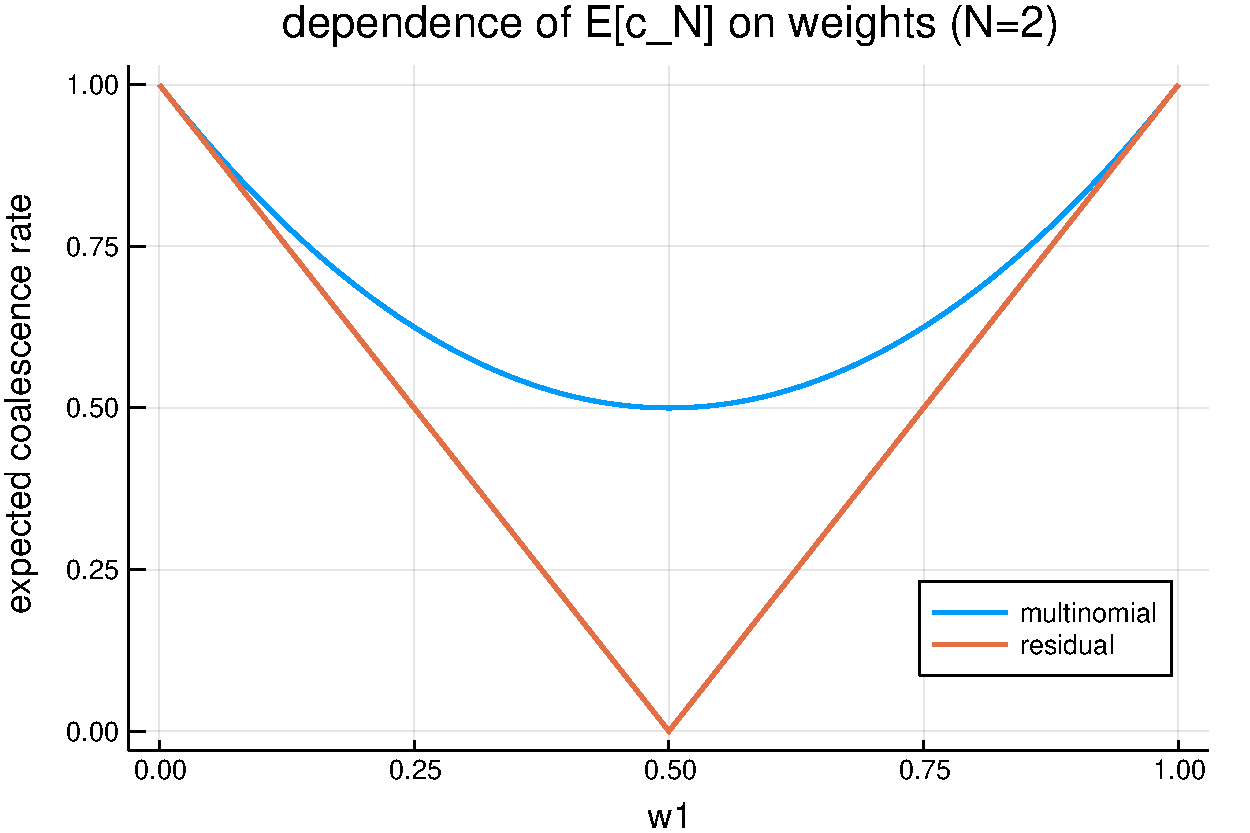
\includegraphics[width=0.8\textwidth]{../residual_resampling/plots/EcN_mn_res_N2.pdf}
\end{center}

%==================

\subsubsection{Case $N=3$}
Given a weight vector $(\wt{1}, \wt{2}, \wt{3})$, let $w_{(1)} \geq w_{(2)} \geq w_{(3)}$ denote the weights sorted from high to low. 
With $N=3$ there are many more cases than with $N=2$, and these are described below, using the sorted weights.

In each case for the conditions on the sorted weights, the possible offspring count vectors (sorted in the same order as the weights) are listed, along with the probability of each (conditional on the given case). Finally, using these outcomes and associated probabilities, the conditional expectation of interest is calculated.\\

\begin{tabular}{ l | l | l | l | l }
Case & Weights & Offspring counts &  Conditional probabilities & $\E[c_2^r(t) | \wt{1:3}]$ \\
\hline
(A) & $w_{(1)} = 1$ & $(3,0,0)$ & 1 & 1 \\
\hline
(B) & $2/3 < w_{(1)} < 1$ & $(3,0,0)$ & $3w_{(1)} - 2$ & $2w_{(1)} -1$\\
	&& $(2,1,0)$ & $3w_{(2)}$ & \\
	&& $(2,0,1)$  & $3w_{(3)}$ & \\
\hline
(C) & $w_{(1)}=2/3$ & $(2,1,0)$ & $3w_{(2)}$ & 1/3 \\
	&& $(2,0,1)$ & $3w_{(3)}$ & \\
\hline
(D1) & $1/3 < w_{(1)} < 2/3$ and & $(2,1,0)$ & $3w_{(1)} - 1$ & $1/3 - w_{(3)}$ \\
	& $1/3 \leq w_{(2)} < 2/3$ & $(1,2,0)$ & $3w_{(2)} -1$ & \\
	&& $(1,1,1)$ & $3w_{(3)}$  & \\
\hline
(D2) &  $1/3 < w_{(1)} < 2/3$ and & $(3,0,0)$ & $(3/2)^2 (w_{(1)} - 1/3)^2$ & $ (1/4) (3w_{(1)} - 1)(w_{(1)} + 1)$ \\
	& $w_{(2)} < 1/3$ & $(2,1,0)$ & $(3/2)^2 2(w_{(1)} - 1/3)w_{(2)}$ &\\
	&& $(2,0,1)$ & $(3/2)^2 2(w_{(1)} - 1/3)w_{(3)}$ &\\
	&& $(1,2,0)$ & $(3/2)^2 w_{(2)}^2$ &\\
	&& $(1,0,2)$ & $(3/2)^2 w_{(3)}^2$ &\\
	&& $(1,1,1)$ & $(3/2)^2 2w_{(2)} w_{(3)}$ &\\
\hline
(E) & $w_{(1)} = 1/3$ & $(1,1,1)$ & 1 & 0 \\
\end{tabular}

\vspace{0.6cm}

\begin{lemma}
For all weight vectors $\wt{1:3}$, 
$\E[c_3^r(t) |\wt{1:3}] \leq \E[c_3^m(t) |\wt{1:3}]$.
\end{lemma}
\begin{proof}
We have the following expression in the case of residual resampling:
\begin{align*}
\E[c_3^r(t) |\wt{1:3}] &= (2w_{(1)} -1) \I{2/3 \leq w_{(1)} \leq 1} \\
&\qquad + (1/3 - w_{(3)}) \I{1/3 \leq w_{(1)} < 2/3} \I{1/3 \leq w_{(2)} < 2/3} \\
&\qquad + (1/4)(3w_{(1)} -1)(w_{(1)} +1) \I{1/3 \leq w_{(1)} < 2/3} \I{w_{(2)} <1/3}
\end{align*}
compared to the following in the case of multinomial resampling:
\begin{align*}
\E[c_3^m(t) |\wt{1:3}] &= w_{(1)}^2 + w_{(2)}^2 + w_{(3)}^2 \\
&= (w_{(1)}^2 + w_{(2)}^2 + w_{(3)}^2) \I{2/3 \leq w_{(1)} \leq 1} \\
&\qquad + (w_{(1)}^2 + w_{(2)}^2 + w_{(3)}^2) \I{1/3 \leq w_{(1)} < 2/3} \I{1/3 \leq w_{(2)} < 2/3} \\
&\qquad + (w_{(1)}^2 + w_{(2)}^2 + w_{(3)}^2) \I{1/3 \leq w_{(1)} < 2/3} \I{w_{(2)} <1/3}.
\end{align*}
Hence it suffices to show the following:
\begin{enumerate}[label=(\roman*)]
\item $(2w_{(1)} -1) \leq (w_{(1)}^2 + w_{(2)}^2 + w_{(3)}^2)$
\item $ (1/3 - w_{(3)}) \leq (w_{(1)}^2 + w_{(2)}^2 + w_{(3)}^2)$
\item $ (1/4)(3w_{(1)} -1)(w_{(1)} +1) \leq (w_{(1)}^2 + w_{(2)}^2 + w_{(3)}^2)$\\
\end{enumerate}
First consider (ii). Since $w_{(3)}$ is defined as the smallest of the three weights, we know that $w_{(3)} \in [0,1/3]$. Meanwhile, the RHS is the sum of the squared weights, which is always between 1/3 and 1. Therefore (ii) is true.\\[7pt]
Now let us consider (i). We have the identity $(w_{(1)} -1)^2 = w_{(1)}^2 -2w_{(1)} +1$, which implies that $w_{(1)}^2 \geq 2_w{(1)} - 1$. Since $w_{(2)}^2 + w_{(3)}^2 \geq 0$ we can therefore conclude that (i) is true.\\[7pt]
Finally consider (iii). In this case it is sufficient to show that $(1/4)(3w_{(1)} -1)(w_{(1)} +1) \leq w_{(1)}^2$. Note that
\begin{align*}
& w_{(1)}^2 - \frac{1}{4}(3w_{(1)} -1)(w_{(1)} +1) \\
& = \frac{1}{4} w_{(1)}^2- \frac{1}{2} w_{(1)} + \frac{1}{4} \\
& = \frac{1}{4} (w_{(1)} -1)^2 \geq 0.
\end{align*}
Therefore (iii) is also true, concluding the proof.
\end{proof}

\begin{figure}
	\centering
	\begin{subfigure}{\textwidth}
		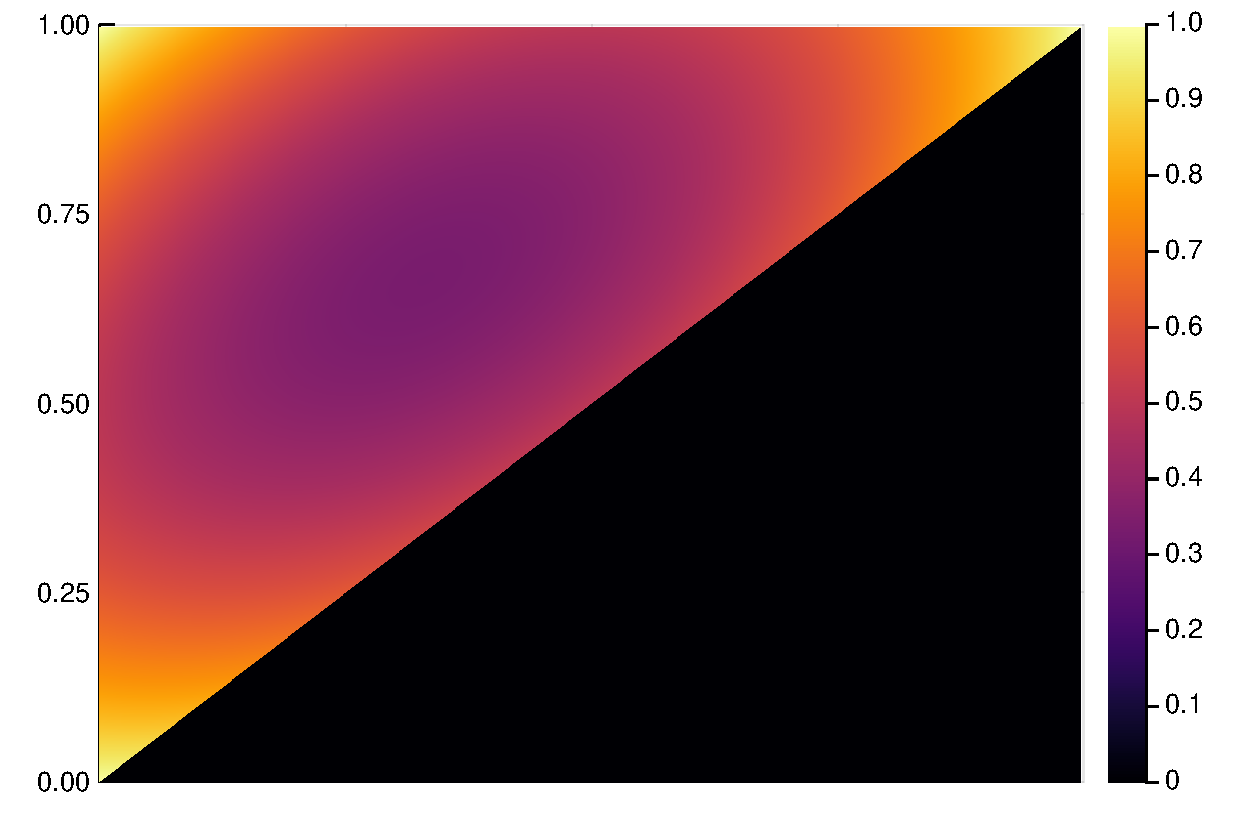
\includegraphics[width=0.5\textwidth]{../residual_resampling/plots/EcN_mn_N3_heatmap.pdf}
		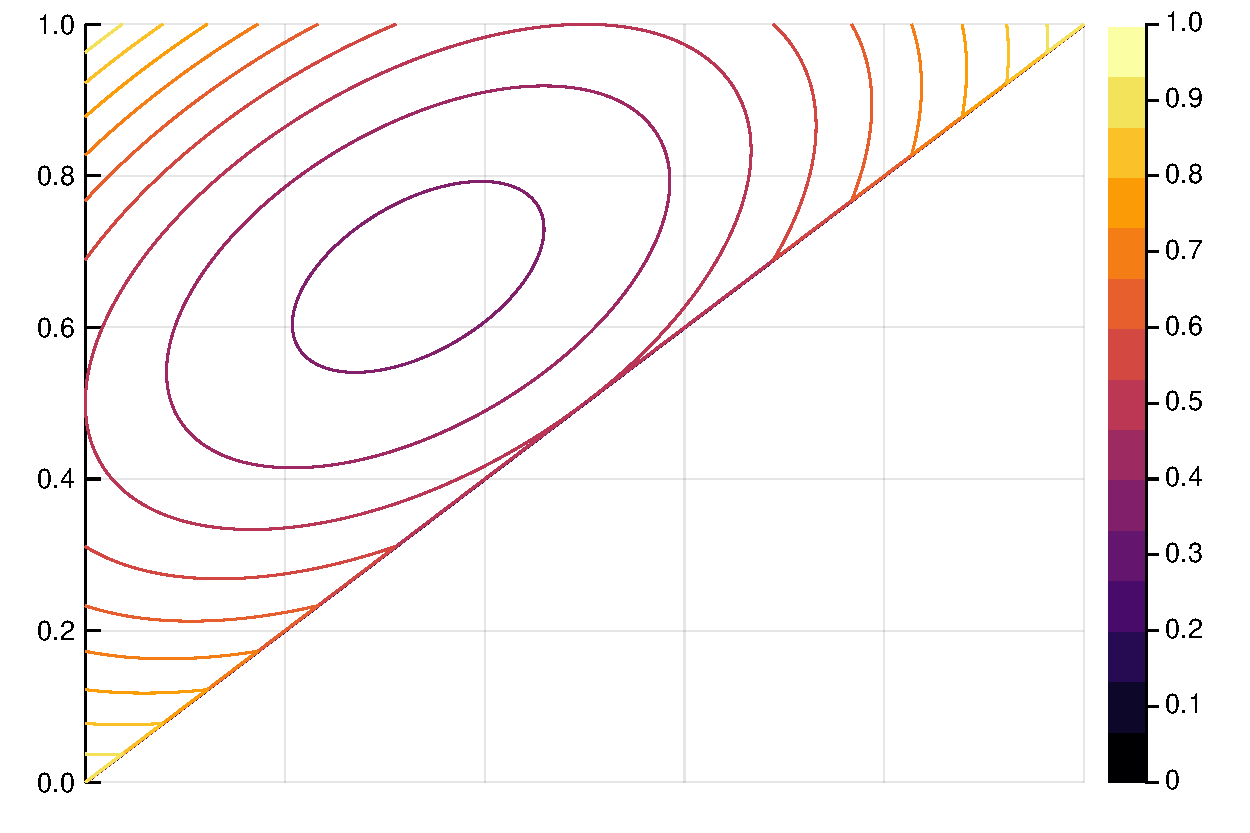
\includegraphics[width=0.5\textwidth]{../residual_resampling/plots/EcN_mn_N3_contour.pdf}
	\caption{Expected coalescence rate with multinomial resampling ($N=3$)}
	\end{subfigure}
	\begin{subfigure}{\textwidth}
		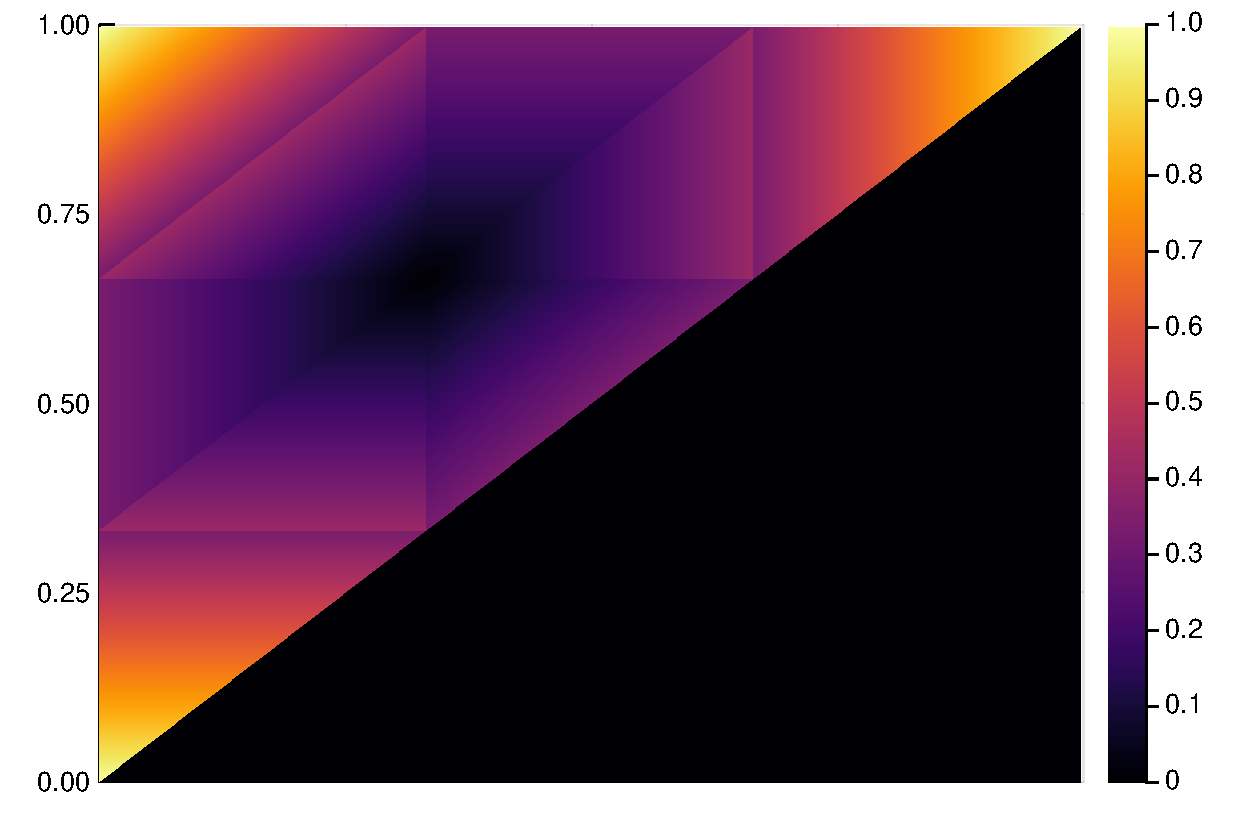
\includegraphics[width=0.5\textwidth]{../residual_resampling/plots/EcN_res_N3_heatmap.pdf}
		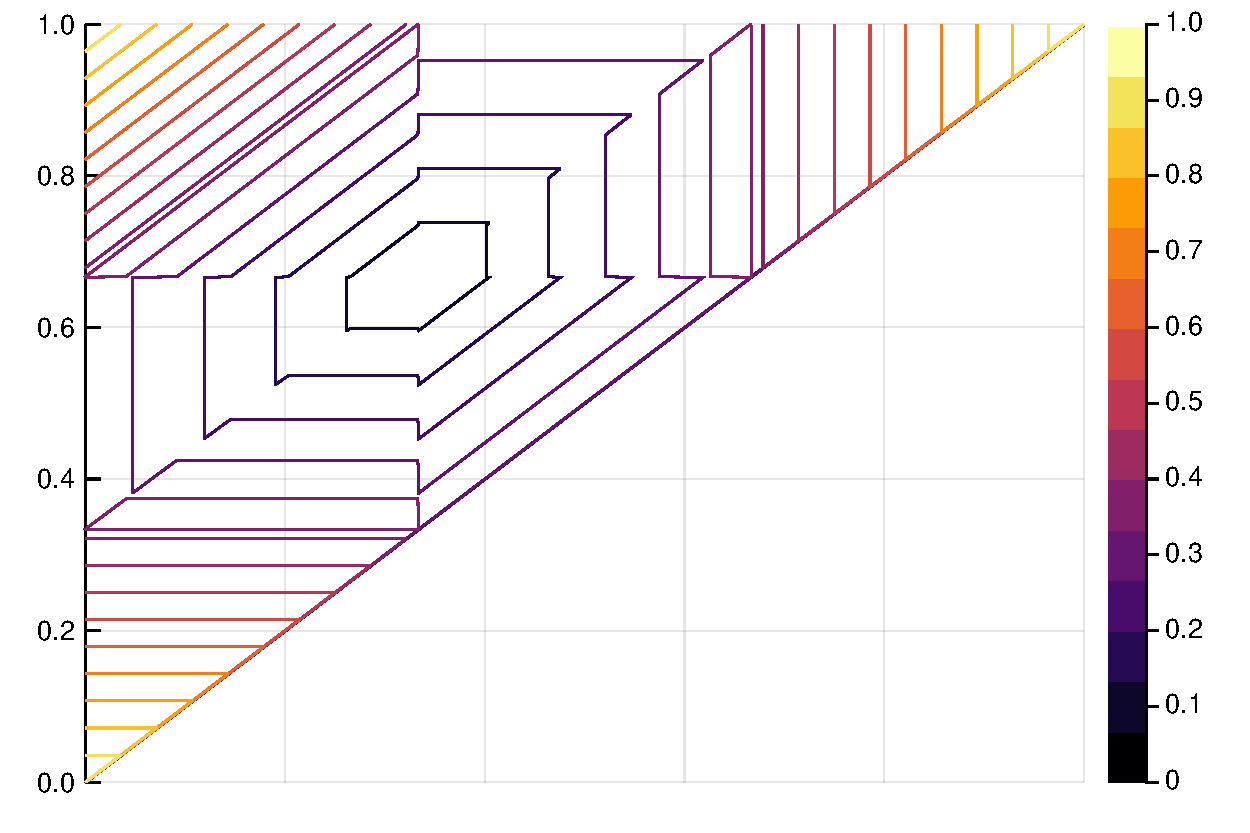
\includegraphics[width=0.5\textwidth]{../residual_resampling/plots/EcN_res_N3_contour.pdf}
	\caption{Expected coalescence rate with residual resampling ($N=3$)}
	\end{subfigure}
	\begin{subfigure}{\textwidth}
		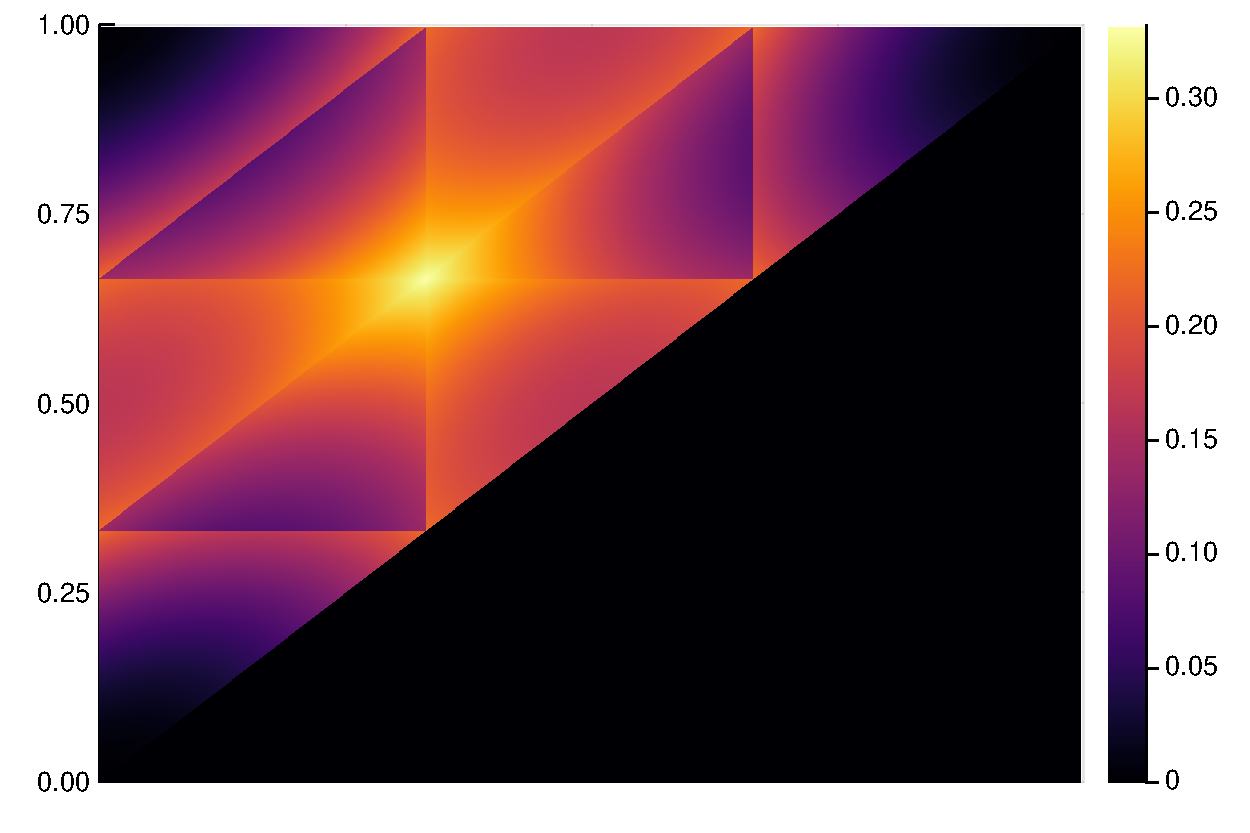
\includegraphics[width=0.5\textwidth]{../residual_resampling/plots/EcN_mn_res_diff_N3_heatmap.pdf}
		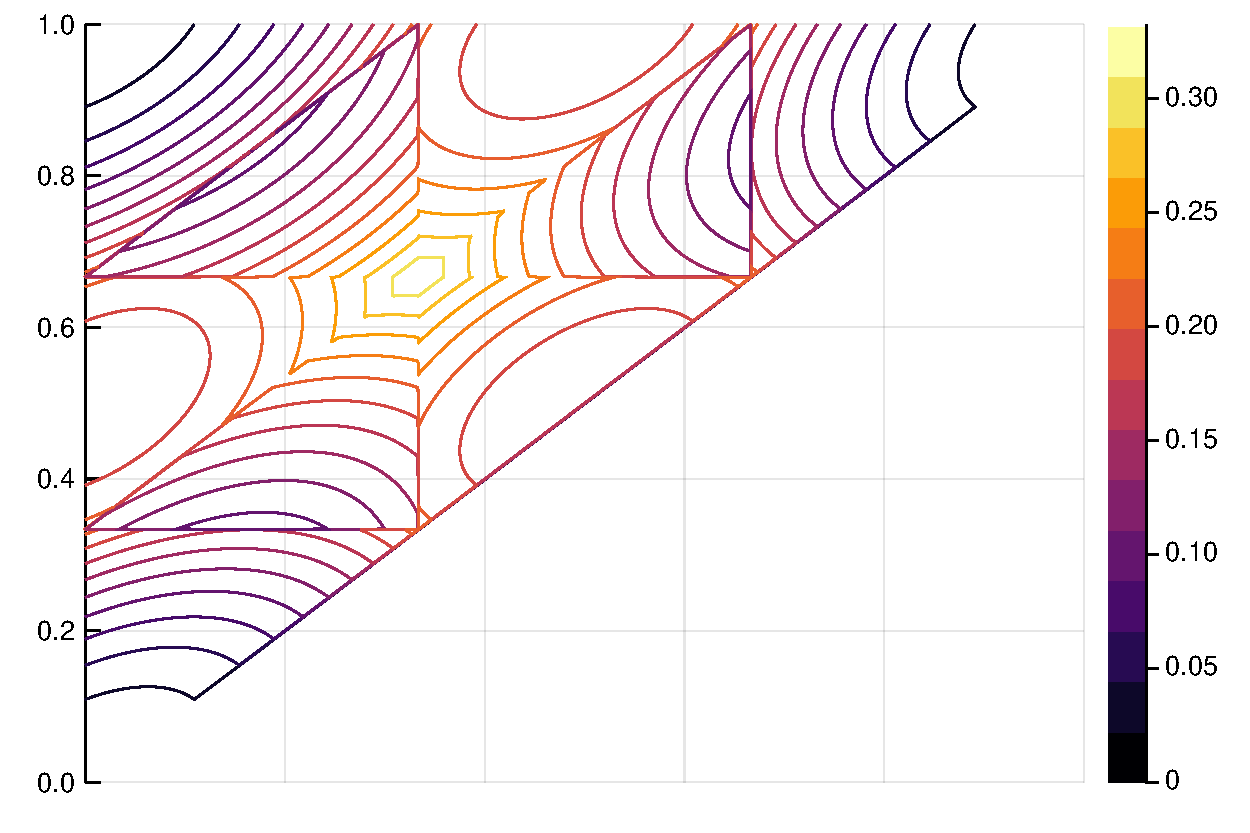
\includegraphics[width=0.5\textwidth]{../residual_resampling/plots/EcN_mn_res_diff_N3_contour.pdf}
	\caption{Difference between expected coalescence rate with multinomial or residual resampling ($N=3$)}
	\end{subfigure}
\end{figure}

\begin{remark}
Examining the table, we can see that the function $\E[c_3^r(t) |\wt{1:3}]$ is continuous in $w_{(1)}$. However, the plot clearly shows discontinuities. These occur at the boundaries between different orderings when we sort the weights from high to low.
\end{remark}

\subsubsection{General $N$}
\begin{lemma}
In the case $w_{(1)} \geq \frac{N-1}{N}$, we have 
\begin{equation*}
\E[c_N^r(t) |\wt{1:N}] = 2w_{(1)} -1.
\end{equation*}
\end{lemma}

\begin{proof}
In this case, (N-1) offspring are deterministically assigned to particle 1. The one remaining offspring can either be assigned to particle 1 or to some other particle.
\begin{itemize}
\item The first option yields offspring vector $(N, 0, 0, \dots)$ and occurs with probability $(w_{(1)} - \frac{N-1}{N})/(1/N) = Nw_{(1)} - (N-1)$. The resulting value of $c_N^r$ is $N(N-1)/(N)_2 = 1$.
\item The second option yields an offspring vector that is some permutation of $(N-1, 1, 0, 0, \dots)$, and occurs with probability $1- Nw_{(1)} - (N-1) = N - Nw_{(1)}$. The resulting value of $c_N^r$ is $(N-1)(N-2)/(N)_2 = (N-2)/N$.
\end{itemize}
So, under this constraint on the weights, we have the following expectation:
\begin{equation*}
\E[c_N^r(t) |\wt{1:N}] = Nw_{(1)} - (N-1) + \frac{N-2}{N}(N - Nw_{(1)}) = 2w_{(1)} -1.
\end{equation*} 
\end{proof}

\begin{lemma}
For $N\geq 3$, in the case $w_{(1)}, w_{(2)}, \dots, w_{(N-1)} \in \left[\frac{1}{N}, \frac{2}{N}\right]$, we have
\begin{equation*}
\E[c_N^r(t) |\wt{1:N}] = \frac{2}{N-1}(1/N - w_{(N)}).
\end{equation*}
\end{lemma}

\begin{proof}
In this case, one offspring is deterministically assigned to each of the particles $1,2,\dots,N-1$. The one remaining offspring can be assigned either to particle $N$ or to one of the others.
\begin{itemize}
\item The first option yields offspring vector $(1,1,\dots, 1)$ and occurs with probability $w_{(N)}/(1/N) = Nw_{(N)}$. The resulting value of $c_N^r$ is 0.
\item The second option yields an offspring vector that is some permutation of $(2,0,1,1,\dots,1)$ and occurs with probability $1- Nw_{(N)}$. The resulting value of $c_N^r$ is 2.
\end{itemize}
So, under this constraint on the weights, we have the following expectation:
\begin{equation*}
\E[c_N^r(t) |\wt{1:N}] = 2(1- Nw_{(N)})/(N)_2 =  \frac{2}{N-1}(1/N - w_{(N)}).
\end{equation*} 
\end{proof}

\begin{conj}
The number of cases to consider for population size $N$ (excluding zero-measure cases which can be included in other cases) is 
\begin{equation*}
p(N-1) + \frac{(N-1)(N-2)}{2}
\end{equation*}
where $p(\cdot)$ denotes the partition function (number of integer partitions).
\end{conj}
This expression was determined by pattern-spotting in low-$N$ cases. I believe a combinatorial proof could be found but, since it is not a particularly useful result, I shan't bother.

\begin{conj}
For all weight vectors $\wt{1:N}$, 
$\E[c_2^m(t) |\wt{1:N}] \geq \E[c_2^r(t) |\wt{1:N}]$.
\end{conj}


\subsection{Squared coalescence rate and other awful expressions}
First let's write down various moments that will be needed (where $i \neq j$).
\begin{align*}
\E[(\vt{i})^2 |\F] &= \flnw^2 + 2\flnw N\wt{i} + (N)_2(\wt{i})^2 \\
\E[(\vt{i})^3 |\F] &= \flnw^3 + 3\flnw^2 N\wt{i} + 3\flnw (N)_2(\wt{i})^2 +(N)_3(\wt{i})^3 \\
\E[(\vt{i})^4 |\F]&= \flnw^4 + 4\flnw^3 N\wt{i} + 6\flnw^2 (N)_2 (\wt{i})^2 + 4\flnw (N)_3(\wt{i})^3 + (N)_4(\wt{i})^4 \\
\E[\vt{i}\vt{j} |\F] &= \flnw\flnw[j] + \flnw N\wt{j} + \flnw[j] N\wt{i} + (N)_2\wt{i}\wt{j} \\
\E[(\vt{i})^2\vt{j} |\F] &= \flnw^2\flnw[j] + \flnw^2 N\wt{j} + 2\flnw\flnw[j] N\wt{i} + 2\flnw (N)_2 \wt{i}\wt{j} \\
&\qquad + \flnw[j] (N)_2(\wt{i})^2 + (N)_3(\wt{i})^2\wt{j}\\
\E[(\vt{i})^2(\vt{j})^2 |\F] &= \flnw^2\flnw[j]^2 +2\flnw^2\flnw[j] N\wt{j} + 2\flnw\flnw[j]^2 N\wt{i} \\
&\qquad + \flnw^2 (N)_2 (\wt{j})^2 + 4\flnw\flnw[j](N)_2\wt{i}\wt{j} + \flnw[j]^2 (N)_2(\wt{i})^2 \\
&\qquad + 2\flnw (N)_3\wt{i}(\wt{j})^2 + 2\flnw[j] (N)_3 (\wt{i})^2\wt{j} + (N)_4 (\wt{i})^2(\wt{j})^2
\end{align*}

For the squared coalescence rate, expanding the falling factorials appropriately, we get
\begin{align*}
\E[(c^r_N(t))^2 |\F] &=
\frac{1}{(N)_2^2} \left( \sum_{i=1}^N \E[(\vt{i})_2^2 |\F] + \sum_{i=1}^N \sum_{j\neq i} \E[(\vt{i})_2 (\vt{j})_2 |\F] \right) \\
&= \frac{1}{(N)_2^2} \sum_{i=1}^N \left( \E[(\vt{i})^4 |\F] - 2 \E[(\vt{i})^3 |\F] + \E[(\vt{i})^2 |\F] \right) \\
&\qquad + \frac{1}{(N)_2^2} \sum_{i=1}^N \sum_{j\neq i} \left( \E[(\vt{i})^2 (\vt{j})^2 |\F] - \E[(\vt{i})^2 \vt{j} |\F] - \E[\vt{i} (\vt{j})^2 |\F] + \E[\vt{i} \vt{j} |\F] \right)
\end{align*}
Then we can try plugging in the expressions derived above and find that none of the terms cancel. Maybe if we're clever we can factorise it or something.

\subsection{Mega-merger rate}
Now the rate of super-binary mergers...
\begin{align*}
\E[D_N(t) |\F] &=
\frac{1}{N(N)_2} \sum_{i=1}^N \left( \E[(\vt{i})^3 |\F] - \E[(\vt{i})^2 |\F] \right) \\
&\qquad + \frac{1}{N(N)_2} \sum_{i=1}^N \sum_{j\neq i} \left( \E[(\vt{i})^2 (\vt{j})^2 |\F] - \E[\vt{i} (\vt{j})^2 |\F] \right)
\end{align*}


\section{Randomised roundings}
\begin{defn}\label{defn:randround_1D}
Let $X\geq0$. A random variable $Y: \mathbb{R}_+ \to \mathbb{N}$ is a \emph{randomised rounding} of $X$ if $Y$ takes the values
\begin{equation*}
Y=
\begin{cases}
 \lfloor X \rfloor & \text{with probability } 1- X+ \lfloor X \rfloor \\
  \lfloor X \rfloor +1 & \text{with probability } X- \lfloor X \rfloor 
\end{cases}
\end{equation*}
\end{defn}
Note that we therefore have $\E[Y] =X$.

Definition \ref{defn:randround_1D} generalises easily to multivariate $X$. A randomised rounding of a vector $X \in \mathbb{R}_+^N$ produces a vector $Y \in \mathbb{N}^N$ such that $\E[Y]=X$. $Y$ can thus be used to construct an unbiased resampling scheme.

Such popular resampling schemes as systematic resampling and residual resampling with systematic residuals are based on randomised roundings. In each scheme, the marginal distributions of the offspring counts are as in Definition \ref{defn:randround_1D}, where $X=N\wt{i}$ and $Y=\vt{i}$. The variety in rounding-based schemes arises from the interactions between these individual offspring counts. 

In this document we will consider a general resampling scheme based on randomised rounding, and compare its genealogical properties to those of multinomial resampling.
Let $(w_1, \dots, w_N)$ be a normalised weight vector (that is, $w_i \geq 0$ and $\sum w_i = 1$), let $N\geq 2$ be an integer denoting the number of particles, and let $(v_1,\dots v_N)$ denote the resampled offspring numbers. We will attach a superscript $m$ or $r$ to denote offspring numbers corresponding to multinomial and rounding-based resampling respectively.

\begin{lemma}
For any $i \in \{1, \dots, N\}$,
\begin{equation*}
\E[(v_i)_2^{(m)} | w_i] \geq \E[(v_i)_2^{(r)} | w_i].
\end{equation*}
\end{lemma}

\begin{proof}
Using properties of the Multinomial distribution \citep{mosimann1962}, we have
\begin{equation*}
\E[(v_i)_2^{(m)} | w_i]  = N(N-1)w_i^2
\end{equation*}
Directly from Definition \ref{defn:randround_1D}, we calculate the corresponding quantity in the case of randomised rounding to be
\begin{align*}
\E[(v_i)_2^{(r)} | w_i] &= \flnw (\flnw -1) (1 - Nw_i + \flnw) + (\flnw +1) \flnw (Nw_i - \flnw) \\
&= \flnw \left( 2(Nw_i - \flnw) + \flnw -1 \right)
\end{align*}
We define the difference 
\begin{align*}
\Delta_i &:= \E[(v_i)_2^{(m)} | w_i] - \E[(v_i)_2^{(r)} | w_i] \\
&= N^2w_i^2 - Nw_i^2 - 2\flnw(Nw_i - \flnw) - \flnw^2 + \flnw \\
&= N^2 w_i^2 + \flnw^2 -2Nw_i \flnw - Nw_i^2 + \flnw \\
&= (Nw_i - \flnw)^2 - Nw_i^2 + \flnw 
\end{align*}
Then we have to show that $\Delta_i \geq 0$ for all $N\geq 2$ and $w_i \in [0,1]$. Consider the following cases.
\begin{description}
\item[Case] $w_i=k/N$ for some $k \in \{1, \dots, N-1\}$. \\
Then $\flnw = Nw_i = k$ and we have\\
$\Delta_i = 0 - k^2/N + k = k(1- k/N) \geq 0$.
\item[Case] $w_i \in (k/N, (k+1)/N )$ for some $k \in \{0, \dots, N-1\}$ \\
Then $\flnw = k$, and
\begin{align*}
\Delta_i &= (Nw_i - k)^2 - Nw_i^2 + k\\
&= N(N-1)w_i^2 - 2Nkw_i + k(k+1) \\
&= N(N-1) \left[ \left( w-\frac{k}{N-1} \right)^2 - \frac{k^2}{(N-1)^2} + \frac{k(k+1)}{N(N-1)} \right]\\
&= N(N-1) \left( w-\frac{k}{N-1} \right)^2 - \frac{k^2 N}{N-1} + k^2 +k \\
&\geq - \frac{k^2 N}{N-1} + k^2 +k \\
&= k\left(1-\frac{k}{N-1}\right)\\
&\geq 0
\end{align*}
\end{description}
For each $N$, any $w_i \in [0,1]$ falls into one of the above cases, so we conclude that $\Delta_i \geq 0$ for all $N, w_i$.
\end{proof}

\begin{figure}
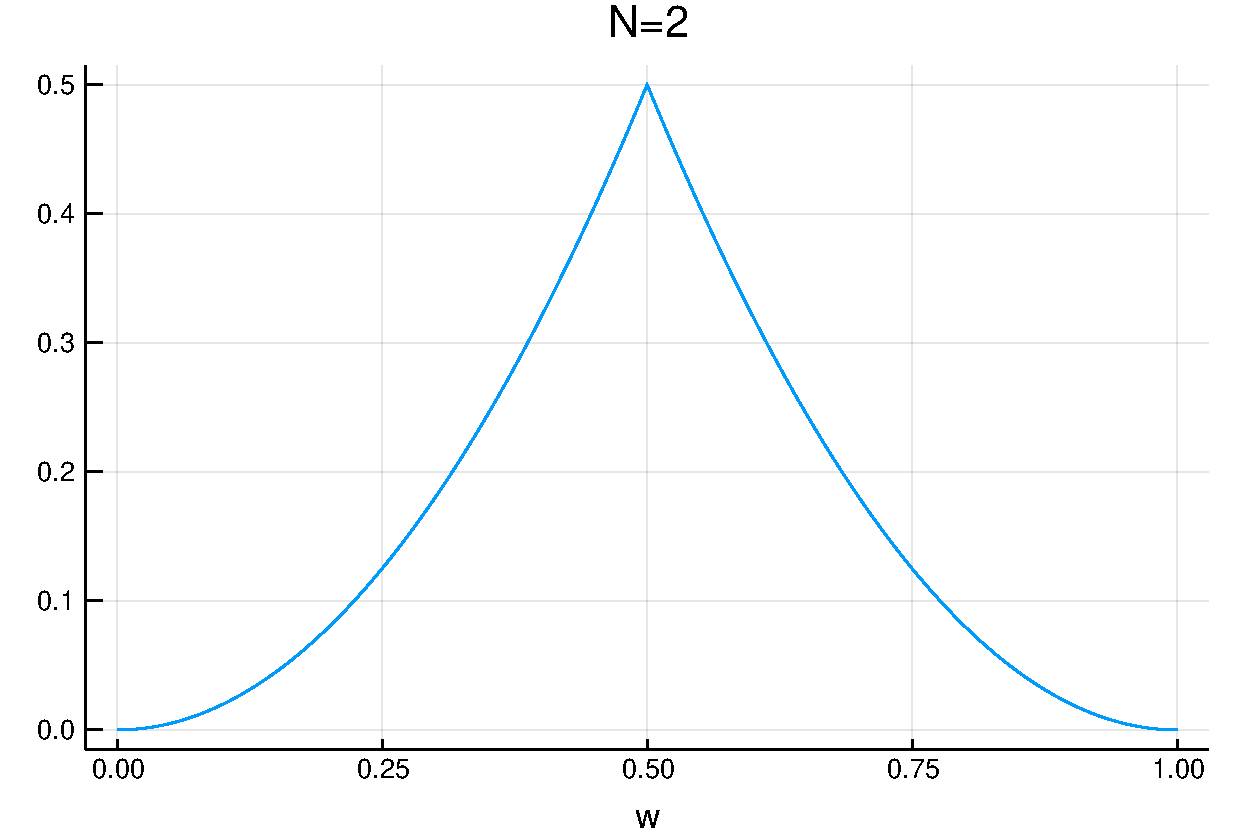
\includegraphics[width=0.33\textwidth]{../randomised_rounding/plots/delta_cN_N2.pdf}
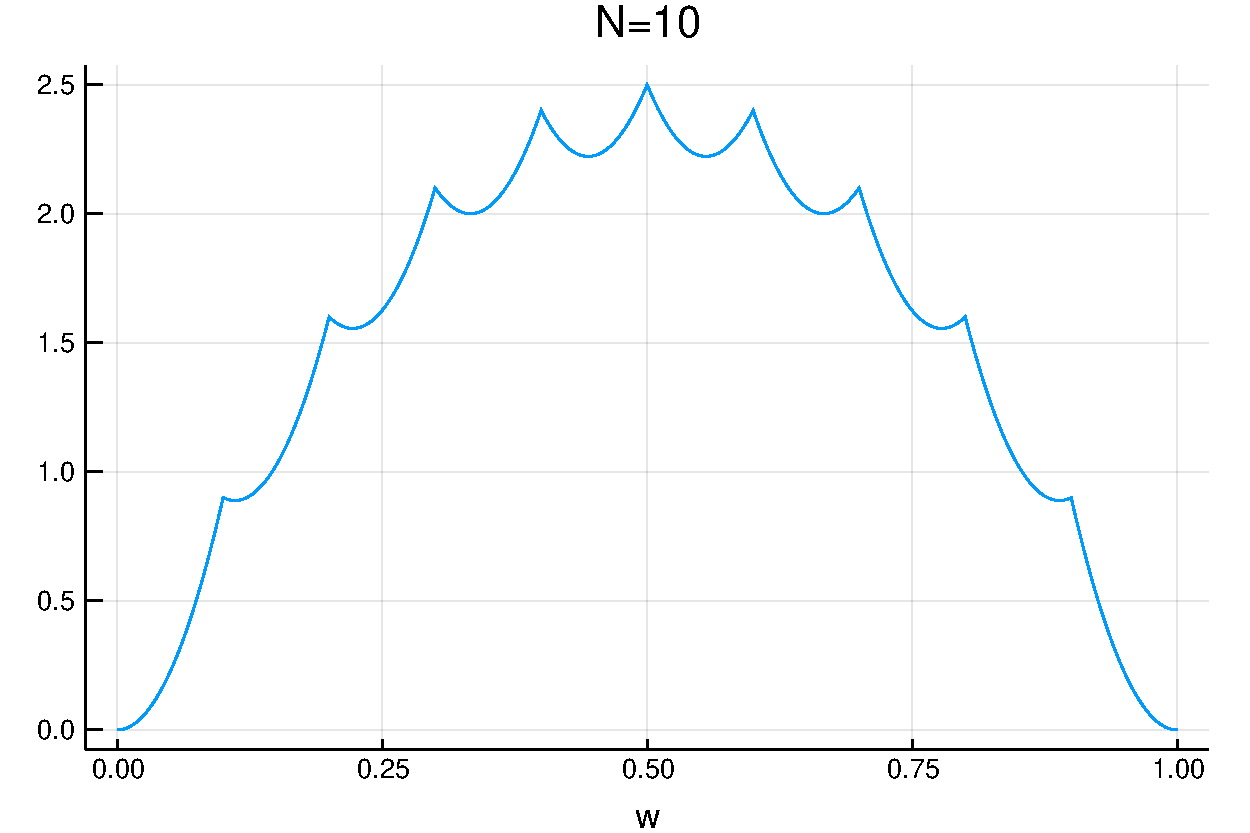
\includegraphics[width=0.33\textwidth]{../randomised_rounding/plots/delta_cN_N10.pdf}
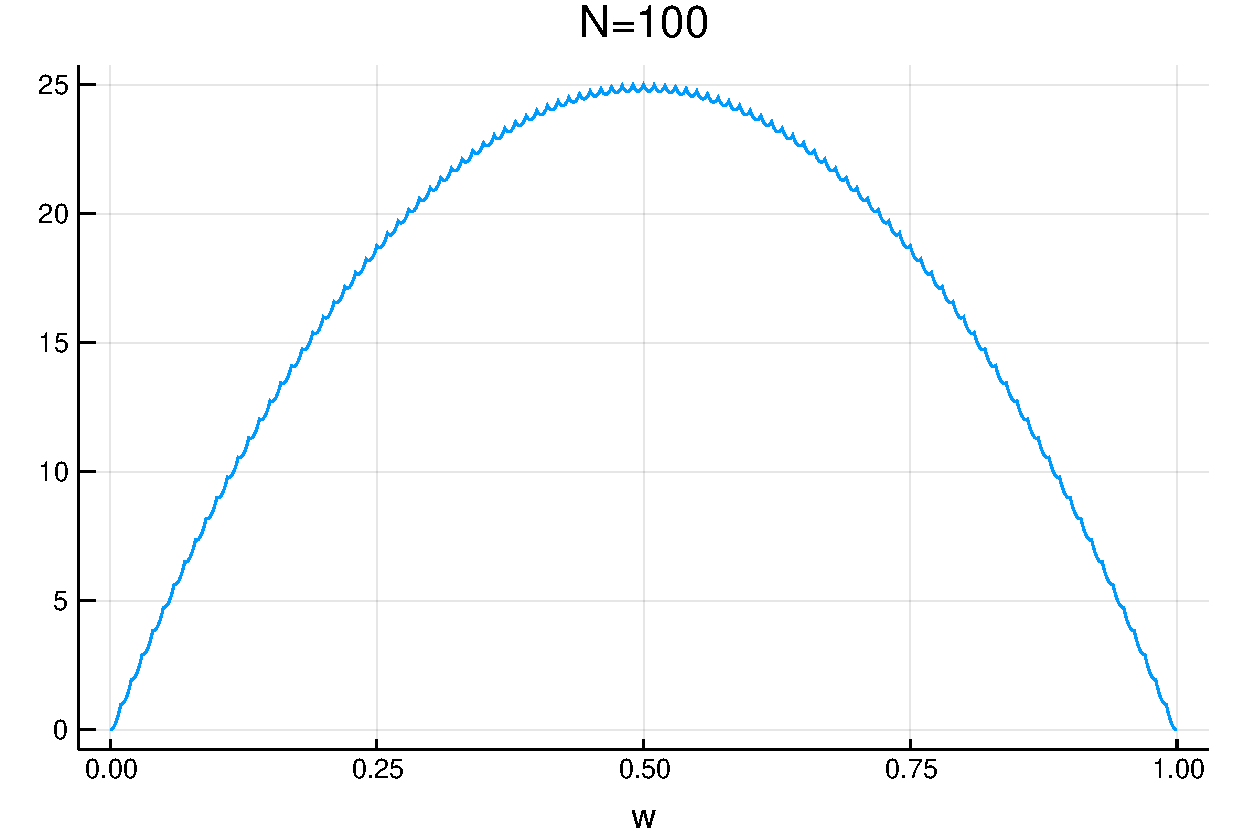
\includegraphics[width=0.33\textwidth]{../randomised_rounding/plots/delta_cN_N100.pdf}
\caption{$\Delta_i$ as a function of $w_i$ for various values of $N$. The function is piecewise quadratic between the points $w_i = k/N$. The limiting shape appears to be a parabola.}
\end{figure}

\bibliography{../smc.bib}
\end{document}